\documentclass[aoas]{imsart}

\RequirePackage{amsthm,amsmath,amsfonts,amssymb}
\RequirePackage[authoryear]{natbib}
\RequirePackage{graphicx}
\RequirePackage{float}
\RequirePackage{placeins}
\RequirePackage[colorlinks,citecolor=blue,urlcolor=blue,linkcolor=blue]{hyperref}

\startlocaldefs
\theoremstyle{definition}
\newtheorem{theorem}{Theorem}
\newtheorem{lemma}[theorem]{Lemma}
\newtheorem{proposition}[theorem]{Proposition}
\newtheorem{corollary}[theorem]{Corollary}
\newtheorem{definition}[theorem]{Definition}
\newtheorem{remark}[theorem]{Remark}
\newcommand{\E}{\mathbb{E}}
\renewcommand{\P}{\mathbb{P}}
\newcommand{\V}{\operatorname{Var}}
% Generated by scripts/manuscript/build-manuscript-artifacts.R; do not edit.
\providecommand{\ChicagoClock}{4:21}
\providecommand{\ChicagoDate}{November 5, 2019}
\providecommand{\ChicagoFinalAwayScore}{118}
\providecommand{\ChicagoFinalHomeScore}{112}
\providecommand{\ChicagoGameID}{401160742}
\providecommand{\ChicagoLoser}{Chicago Bulls}
\providecommand{\ChicagoMaxWP}{96.9\%}
\providecommand{\ChicagoMinutesRemaining}{16.4}
\providecommand{\ChicagoPIT}{0.968}
\providecommand{\ChicagoPeakAwayScore}{67}
\providecommand{\ChicagoPeakHomeScore}{85}
\providecommand{\ChicagoPeakLead}{18}
\providecommand{\ChicagoPeriod}{3}
\providecommand{\ChicagoSeason}{2020}
\providecommand{\ChicagoStartingWP}{71.2\%}
\providecommand{\ChicagoTailProbability}{3.2\%}
\providecommand{\ChicagoWinner}{Los Angeles Lakers}
\providecommand{\DyadicBootstrapReplicates}{9,999}
\providecommand{\DyadicBootstrapSeed}{20260815}
\providecommand{\NBACompletedGames}{8,290}
\providecommand{\NBACoverageRows}{
2018 & 1,230 & 1,230 & 1,222 & 8 \\
2019 & 1,230 & 1,230 & 1,230 & 0 \\
2020 & 1,062 & 1,059 & 1,053 & 6 \\
2021 & 1,112 & 1,080 & 1,080 & 0 \\
2022 & 1,241 & 1,230 & 1,230 & 0 \\
2023 & 1,231 & 1,230 & 1,230 & 0 \\
2024 & 1,233 & 1,231 & 1,231 & 0 \\
}
\providecommand{\NBACrossingNinetyCILower}{2.7\%}
\providecommand{\NBACrossingNinetyCIUpper}{4.7\%}
\providecommand{\NBACrossingNinetyEpisodes}{9,371}
\providecommand{\NBACrossingNinetyFiveAllCILower}{1.4\%}
\providecommand{\NBACrossingNinetyFiveAllCIUpper}{3.1\%}
\providecommand{\NBACrossingNinetyFiveAllEpisodes}{8,829}
\providecommand{\NBACrossingNinetyFiveAllGames}{8,266}
\providecommand{\NBACrossingNinetyFiveAllImplied}{4.1\%}
\providecommand{\NBACrossingNinetyFiveAllLoss}{6.4\%}
\providecommand{\NBACrossingNinetyFiveAllResidual}{2.3\%}
\providecommand{\NBACrossingNinetyFiveCILower}{1.4\%}
\providecommand{\NBACrossingNinetyFiveCIUpper}{3.2\%}
\providecommand{\NBACrossingNinetyFiveEpisodes}{8,663}
\providecommand{\NBACrossingNinetyFiveGames}{8,156}
\providecommand{\NBACrossingNinetyFiveImplied}{4.2\%}
\providecommand{\NBACrossingNinetyFiveLoss}{6.5\%}
\providecommand{\NBACrossingNinetyFiveResidual}{2.3\%}
\providecommand{\NBACrossingNinetyFiveStrictCILower}{1.5\%}
\providecommand{\NBACrossingNinetyFiveStrictCIUpper}{3.2\%}
\providecommand{\NBACrossingNinetyFiveStrictEpisodes}{8,654}
\providecommand{\NBACrossingNinetyFiveStrictGames}{8,154}
\providecommand{\NBACrossingNinetyFiveStrictImplied}{4.1\%}
\providecommand{\NBACrossingNinetyFiveStrictLoss}{6.4\%}
\providecommand{\NBACrossingNinetyFiveStrictResidual}{2.3\%}
\providecommand{\NBACrossingNinetyGames}{8,250}
\providecommand{\NBACrossingNinetyImplied}{8.8\%}
\providecommand{\NBACrossingNinetyLoss}{12.5\%}
\providecommand{\NBACrossingNinetyNineCILower}{0.1\%}
\providecommand{\NBACrossingNinetyNineCIUpper}{0.9\%}
\providecommand{\NBACrossingNinetyNineEpisodes}{7,660}
\providecommand{\NBACrossingNinetyNineGames}{7,598}
\providecommand{\NBACrossingNinetyNineImplied}{0.8\%}
\providecommand{\NBACrossingNinetyNineLoss}{1.3\%}
\providecommand{\NBACrossingNinetyNineResidual}{0.5\%}
\providecommand{\NBACrossingNinetyResidual}{3.7\%}
\providecommand{\NBADyadicCalendarGlobalD}{0.097}
\providecommand{\NBADyadicCalendarGlobalP}{\ensuremath{<0.001}}
\providecommand{\NBAEligibleGames}{8,290}
\providecommand{\NBAExcludePatchedGlobalD}{0.096}
\providecommand{\NBAExcludePatchedGlobalP}{\ensuremath{<0.001}}
\providecommand{\NBAExcludedExhibitionEvents}{10}
\providecommand{\NBAExcludedExhibitionFeeds}{5}
\providecommand{\NBAFixedClockExcluded}{11}
\providecommand{\NBAFixedClockGames}{8,265}
\providecommand{\NBAFixedClockLOCFCells}{195}
\providecommand{\NBAFixedClockLOCFRMS}{2.8\%}
\providecommand{\NBAFixedClockLOCFSignificantCells}{3}
\providecommand{\NBAFixedClockLinearCells}{196}
\providecommand{\NBAFixedClockLinearRMS}{2.7\%}
\providecommand{\NBAFixedClockLinearSignificantCells}{2}
\providecommand{\NBAFranchiseLinkedGlobalD}{0.097}
\providecommand{\NBAFranchiseLinkedGlobalP}{\ensuremath{<0.001}}
\providecommand{\NBAGames}{8,276}
\providecommand{\NBAGlobalCritical}{0.023}
\providecommand{\NBAGlobalD}{0.097}
\providecommand{\NBAGlobalDyadicP}{\ensuremath{<0.001}}
\providecommand{\NBALOSODMax}{0.102}
\providecommand{\NBALOSODMin}{0.093}
\providecommand{\NBALOSOTailMax}{1.5\%}
\providecommand{\NBALOSOTailMin}{1.2\%}
\providecommand{\NBALeaveSeasonRows}{
2018 & 7,054 & 0.093 & 1.5\% \\
2019 & 7,046 & 0.097 & 1.2\% \\
2020 & 7,223 & 0.094 & 1.3\% \\
2021 & 7,196 & 0.100 & 1.3\% \\
2022 & 7,046 & 0.102 & 1.3\% \\
2023 & 7,046 & 0.093 & 1.2\% \\
2024 & 7,045 & 0.101 & 1.5\% \\
}
\providecommand{\NBAMedianUpdatesPerGame}{466}
\providecommand{\NBAMinimumFeedCoverage}{99.3\%}
\providecommand{\NBAMissingCoverageRows}{
2018 & 1,222 & 8 & 99.3\% \\
2019 & 1,230 & 0 & 100.0\% \\
2020 & 1,053 & 6 & 99.4\% \\
2021 & 1,080 & 0 & 100.0\% \\
2022 & 1,230 & 0 & 100.0\% \\
2023 & 1,230 & 0 & 100.0\% \\
2024 & 1,231 & 0 & 100.0\% \\
}
\providecommand{\NBAMissingFeedGames}{14}
\providecommand{\NBANonfinalGames}{49}
\providecommand{\NBAPatchedGames}{16}
\providecommand{\NBAPublishedUpdates}{3,877,820}
\providecommand{\NBARawGlobalD}{0.097}
\providecommand{\NBARawGlobalP}{\ensuremath{<0.001}}
\providecommand{\NBARoundingLowerGlobalD}{0.095}
\providecommand{\NBARoundingLowerGlobalP}{\ensuremath{<0.001}}
\providecommand{\NBARoundingLowerTailNinetyFiveRate}{6.3\%}
\providecommand{\NBARoundingUpperGlobalD}{0.099}
\providecommand{\NBARoundingUpperGlobalP}{\ensuremath{<0.001}}
\providecommand{\NBARoundingUpperTailNinetyFiveRate}{6.6\%}
\providecommand{\NBAScheduledGames}{8,339}
\providecommand{\NBATailNinetyCILower}{1.4\%}
\providecommand{\NBATailNinetyCIUpper}{4.0\%}
\providecommand{\NBATailNinetyExcess}{2.7\%}
\providecommand{\NBATailNinetyFiveAtomRate}{0.00\%}
\providecommand{\NBATailNinetyFiveCILower}{0.4\%}
\providecommand{\NBATailNinetyFiveCIUpper}{2.3\%}
\providecommand{\NBATailNinetyFiveExcess}{1.3\%}
\providecommand{\NBATailNinetyFiveRate}{6.3\%}
\providecommand{\NBATailNinetyFiveStrictRate}{6.3\%}
\providecommand{\NBATailNinetyNineCILower}{-0.3\%}
\providecommand{\NBATailNinetyNineCIUpper}{0.5\%}
\providecommand{\NBATailNinetyNineExcess}{0.1\%}
\providecommand{\NBATailNinetyNineRate}{1.1\%}
\providecommand{\NBATailNinetyRate}{12.7\%}
\providecommand{\NBATiedGames}{0}
\providecommand{\NBAUpdateQOne}{447}
\providecommand{\NBAUpdateQThree}{488}
\providecommand{\NFLCompletedGames}{1,855}
\providecommand{\NFLCoverageRows}{
2018 & 256 & 254 & 254 & 0 \\
2019 & 256 & 255 & 255 & 0 \\
2020 & 256 & 255 & 255 & 0 \\
2021 & 272 & 271 & 271 & 0 \\
2022 & 272 & 269 & 269 & 0 \\
2023 & 272 & 272 & 272 & 0 \\
2024 & 272 & 272 & 272 & 0 \\
}
\providecommand{\NFLCrossingNinetyCILower}{-0.9\%}
\providecommand{\NFLCrossingNinetyCIUpper}{2.8\%}
\providecommand{\NFLCrossingNinetyEpisodes}{1,974}
\providecommand{\NFLCrossingNinetyFiveAllCILower}{-0.2\%}
\providecommand{\NFLCrossingNinetyFiveAllCIUpper}{2.7\%}
\providecommand{\NFLCrossingNinetyFiveAllEpisodes}{1,932}
\providecommand{\NFLCrossingNinetyFiveAllGames}{1,847}
\providecommand{\NFLCrossingNinetyFiveAllImplied}{3.2\%}
\providecommand{\NFLCrossingNinetyFiveAllLoss}{4.4\%}
\providecommand{\NFLCrossingNinetyFiveAllResidual}{1.2\%}
\providecommand{\NFLCrossingNinetyFiveCILower}{-0.2\%}
\providecommand{\NFLCrossingNinetyFiveCIUpper}{2.9\%}
\providecommand{\NFLCrossingNinetyFiveEpisodes}{1,842}
\providecommand{\NFLCrossingNinetyFiveGames}{1,772}
\providecommand{\NFLCrossingNinetyFiveImplied}{3.3\%}
\providecommand{\NFLCrossingNinetyFiveLoss}{4.6\%}
\providecommand{\NFLCrossingNinetyFiveResidual}{1.3\%}
\providecommand{\NFLCrossingNinetyFiveStrictCILower}{-0.2\%}
\providecommand{\NFLCrossingNinetyFiveStrictCIUpper}{2.9\%}
\providecommand{\NFLCrossingNinetyFiveStrictEpisodes}{1,841}
\providecommand{\NFLCrossingNinetyFiveStrictGames}{1,771}
\providecommand{\NFLCrossingNinetyFiveStrictImplied}{3.3\%}
\providecommand{\NFLCrossingNinetyFiveStrictLoss}{4.6\%}
\providecommand{\NFLCrossingNinetyFiveStrictResidual}{1.3\%}
\providecommand{\NFLCrossingNinetyGames}{1,818}
\providecommand{\NFLCrossingNinetyImplied}{7.6\%}
\providecommand{\NFLCrossingNinetyLoss}{8.5\%}
\providecommand{\NFLCrossingNinetyNineCILower}{0.2\%}
\providecommand{\NFLCrossingNinetyNineCIUpper}{2.2\%}
\providecommand{\NFLCrossingNinetyNineEpisodes}{1,705}
\providecommand{\NFLCrossingNinetyNineGames}{1,686}
\providecommand{\NFLCrossingNinetyNineImplied}{0.5\%}
\providecommand{\NFLCrossingNinetyNineLoss}{1.6\%}
\providecommand{\NFLCrossingNinetyNineResidual}{1.1\%}
\providecommand{\NFLCrossingNinetyResidual}{0.9\%}
\providecommand{\NFLDyadicCalendarGlobalD}{0.015}
\providecommand{\NFLDyadicCalendarGlobalP}{\ensuremath{0.856}}
\providecommand{\NFLEligibleGames}{1,848}
\providecommand{\NFLExcludePatchedGlobalD}{0.014}
\providecommand{\NFLExcludePatchedGlobalP}{\ensuremath{0.769}}
\providecommand{\NFLFixedClockExcluded}{0}
\providecommand{\NFLFixedClockGames}{1,848}
\providecommand{\NFLFixedClockLOCFCells}{197}
\providecommand{\NFLFixedClockLOCFRMS}{2.6\%}
\providecommand{\NFLFixedClockLOCFSignificantCells}{8}
\providecommand{\NFLFixedClockLinearCells}{197}
\providecommand{\NFLFixedClockLinearRMS}{2.9\%}
\providecommand{\NFLFixedClockLinearSignificantCells}{8}
\providecommand{\NFLFranchiseLinkedGlobalD}{0.015}
\providecommand{\NFLFranchiseLinkedGlobalP}{\ensuremath{0.705}}
\providecommand{\NFLGames}{1,848}
\providecommand{\NFLGlobalCritical}{0.047}
\providecommand{\NFLGlobalD}{0.015}
\providecommand{\NFLGlobalDyadicP}{\ensuremath{0.736}}
\providecommand{\NFLLOSODMax}{0.025}
\providecommand{\NFLLOSODMin}{0.008}
\providecommand{\NFLLOSOTailMax}{0.0\%}
\providecommand{\NFLLOSOTailMin}{-1.0\%}
\providecommand{\NFLLeaveSeasonRows}{
2018 & 1,594 & 0.017 & -0.7\% \\
2019 & 1,593 & 0.013 & -0.3\% \\
2020 & 1,593 & 0.014 & -1.0\% \\
2021 & 1,577 & 0.013 & -0.3\% \\
2022 & 1,579 & 0.008 & -0.8\% \\
2023 & 1,576 & 0.024 & -0.4\% \\
2024 & 1,576 & 0.025 & 0.0\% \\
}
\providecommand{\NFLMedianUpdatesPerGame}{175}
\providecommand{\NFLMinimumFeedCoverage}{100.0\%}
\providecommand{\NFLMissingCoverageRows}{
2018 & 254 & 0 & 100.0\% \\
2019 & 255 & 0 & 100.0\% \\
2020 & 255 & 0 & 100.0\% \\
2021 & 271 & 0 & 100.0\% \\
2022 & 269 & 0 & 100.0\% \\
2023 & 272 & 0 & 100.0\% \\
2024 & 272 & 0 & 100.0\% \\
}
\providecommand{\NFLMissingFeedGames}{0}
\providecommand{\NFLNonfinalGames}{1}
\providecommand{\NFLPatchedGames}{4}
\providecommand{\NFLPublishedUpdates}{325,922}
\providecommand{\NFLRawGlobalD}{0.015}
\providecommand{\NFLRawGlobalP}{\ensuremath{0.735}}
\providecommand{\NFLRoundingLowerGlobalD}{0.013}
\providecommand{\NFLRoundingLowerGlobalP}{\ensuremath{0.775}}
\providecommand{\NFLRoundingLowerTailNinetyFiveRate}{4.5\%}
\providecommand{\NFLRoundingUpperGlobalD}{0.016}
\providecommand{\NFLRoundingUpperGlobalP}{\ensuremath{0.679}}
\providecommand{\NFLRoundingUpperTailNinetyFiveRate}{4.5\%}
\providecommand{\NFLScheduledGames}{1,856}
\providecommand{\NFLTailNinetyCILower}{-3.5\%}
\providecommand{\NFLTailNinetyCIUpper}{0.7\%}
\providecommand{\NFLTailNinetyExcess}{-1.5\%}
\providecommand{\NFLTailNinetyFiveAtomRate}{0.00\%}
\providecommand{\NFLTailNinetyFiveCILower}{-2.0\%}
\providecommand{\NFLTailNinetyFiveCIUpper}{1.1\%}
\providecommand{\NFLTailNinetyFiveExcess}{-0.5\%}
\providecommand{\NFLTailNinetyFiveRate}{4.5\%}
\providecommand{\NFLTailNinetyFiveStrictRate}{4.5\%}
\providecommand{\NFLTailNinetyNineCILower}{-0.3\%}
\providecommand{\NFLTailNinetyNineCIUpper}{1.5\%}
\providecommand{\NFLTailNinetyNineExcess}{0.5\%}
\providecommand{\NFLTailNinetyNineRate}{1.5\%}
\providecommand{\NFLTailNinetyRate}{8.5\%}
\providecommand{\NFLTiedGames}{7}
\providecommand{\NFLUpdateQOne}{167}
\providecommand{\NFLUpdateQThree}{185}
\providecommand{\SimulationBaseGrid}{1,000}
\providecommand{\SimulationCoarseningN}{50,000}
\providecommand{\ValidationInnerReplicates}{399}
\providecommand{\ValidationNBARhoFiftyDyadic}{4.4\%}
\providecommand{\ValidationNBARhoTwentyFiveDyadic}{3.2\%}
\providecommand{\ValidationNBARhoZeroDyadic}{0.0\%}
\providecommand{\ValidationNFLRhoFiftyDyadic}{3.2\%}
\providecommand{\ValidationNFLRhoTwentyFiveDyadic}{0.8\%}
\providecommand{\ValidationNFLRhoZeroDyadic}{0.0\%}
\providecommand{\ValidationOuterSamples}{250}
\endlocaldefs

\begin{document}
\begin{frontmatter}
\title{The Blown Lead Paradox: A Pathwise Calibration Benchmark for Win Probability Forecasts}
\runtitle{The Blown Lead Paradox}

\begin{aug}
\author[A]{\fnms{Jonathan}~\snm{Pipping-Gam\'on}\ead[label=e1]{jpipping@wharton.upenn.edu}\orcid{0009-0000-2540-2469}}
\and
\author[A]{\fnms{Abraham J.}~\snm{Wyner}\ead[label=e2]{ajw@wharton.upenn.edu}}
\address[A]{Department of Statistics, University of Pennsylvania \printead[presep={,\ }]{e1,e2}}
\end{aug}

\begin{abstract}
Live win probabilities have given sports collapses a common numerical language: the highest win probability attained by the team that eventually lost. Yet this familiar number is a selected pathwise extreme. The losing path is identified by the terminal outcome and then searched for its most favorable point. Under ideal sequential calibration, we derive an exact continuous-path benchmark for this statistic, a conservative bound for discretely reported paths, and a probability-integral-transform diagnostic for collections of games. Unlike fixed-time calibration summaries and proper scores, the diagnostic asks whether a published feed produces severe losing paths as often as a calibrated sequential model should. We apply the benchmark separately to public regular-season NFL and NBA feeds from 2018--2024, using a season-stratified dyadic bootstrap to account for recurring teams. We detect no global departure in the NFL and a systematic excess of extreme losing-team peaks in the NBA\@. In the upper 5\% benchmark tail, the NBA excess is \NBATailNinetyFiveExcess{} (95\% interval \NBATailNinetyFiveCILower{} to \NBATailNinetyFiveCIUpper{}); first crossings of a published win probability of $0.95$ show the same positive gap between observed and implied loss rates.
\end{abstract}

\begin{keyword}
\raggedright
\kwd{\mbox{Forecast calibration}}
\kwd{martingales}
\kwd[,\newline]{\mbox{pigeonhole bootstrap}}
\kwd{\mbox{sports analytics}}
\kwd{\mbox{win probability}}
\end{keyword}
\end{frontmatter}

\section{Introduction}

On \ChicagoDate, with \ChicagoClock{} remaining in the third quarter, the Chicago Bulls led the Los Angeles Lakers \ChicagoPeakHomeScore--\ChicagoPeakAwayScore{}.
ESPN's win probability feed put Chicago's chance of winning at \ChicagoMaxWP{}; the Bulls went on to lose \ChicagoFinalHomeScore--\ChicagoFinalAwayScore{} \citep{ESPN2019BullsLakers}.
After the final whistle, that one number became a natural summary of the collapse.
This is the appeal of win probability: a basketball lead of \ChicagoPeakLead{} points and a two-score football lead are not directly comparable on the scoreboard, but both can be expressed on the same probability scale.
Modern accounts of blown leads therefore often report the highest win probability reached by the team that eventually lost.

That convenience hides a conditioning problem.
When the \ChicagoMaxWP{} forecast was issued, its complement described Chicago's conditional chance of losing under the model.
After the game, however, Chicago was selected precisely because it lost, and its path was then searched for its most favorable point.
The complement of the selected maximum is not the frequency with which calibrated losing paths should reach a maximum that high.
Answering the retrospective question requires a different benchmark: among calibrated paths that end in defeat, how large should the losing team's maximum be?

For a two-team game, we study the largest win probability attained by whichever team eventually loses.
The terminal outcome selects one team's path, and the reported sequence supplies its observed peak.
This quantity is easy to read from a game graphic but less easy to judge, because its comparison class consists of losing paths rather than all forecasts made at a fixed probability.
If an eventual loser once reached $95\%$, the relevant question is not simply whether $5\%$ events occur.
It is how often a calibrated sequential model produces losing paths with peaks at or above $95\%$.

Let $Y\in\{0,1\}$ indicate whether Team~A wins.
Our reference model is ideal sequential calibration:
\[
p_k=\P(Y=1\mid \mathcal F_k),\qquad k=0,1,\dots,N,
\]
under which the forecast is a bounded martingale ending at $p_N=Y$.
This ideal is stronger than marginal calibration within probability bins: every probability must equal the conditional chance of winning given the information then available, so the sequence is dynamically coherent.
That martingale structure yields an exact benchmark for continuously observed paths and a conservative one for discretely reported paths.
It also turns each game into a common benchmark score that can be aggregated across a league.

The resulting diagnostic adds a pathwise question to ordinary forecast evaluation.
Reliability diagrams ask whether events forecast near $p$ occur about $p$ of the time, while Brier and log scores summarize predictive performance across individual forecasts \citep{Brier1950,Murphy1973,DeGrootFienberg1983,Dawid1982,GneitingRaftery2007}.
These tools evaluate individual forecasts; the blown-lead statistic evaluates a maximum chosen after the losing team is known.
A feed can look broadly reliable update by update and still produce too many extreme losing-team maxima, or the reverse.

That distinction connects two strands of earlier work.
Sports statisticians have modeled in-game win probability through score-evolution models \citep{Stern1994} and play-level machine-learning methods \citep{LockNettleton2014,YurkoVenturaHorowitz2019}.
Most directly, \citet{YehRiceDubin2022} developed calibration surfaces and comparative tests for continuously updated NBA forecasts and found ESPN's published feed broadly calibrated at the update level.
Their result makes the pathwise question sharper: can a feed whose individual updates look reasonable nevertheless produce too many extreme maxima among eventual losers?
The sequential-forecasting literature supplies the martingale and prequential language for asking that question \citep{Dawid1984,FosterVohra1998}, while recent work provides broader tests of sequential calibration \citep[e.g.,][]{Howard2020,RamdasGrunwaldVovkShafer2023,ArnoldHenziZiegel2023}.

The remaining obstacle is the reverse conditioning built into a blown lead.
Doob- and Ville-type inequalities control unconditional events such as $\{\sup_t p_t\ge x\}$, but the sports question selects paths that end in failure.
Exact identities for martingale suprema are known in related continuous-time settings \citep{NikeghbaliYor2006}.
Specializing that logic to bounded martingales with binary terminal values gives a closed-form law for the losing team's maximum, along with corrections for discrete reporting.

The empirical applications use public regular-season NFL and NBA win probability feeds from 2018--2024.
To account for recurring teams and matchups, we use a season-stratified dyadic pigeonhole bootstrap across \NFLGames{} NFL games and \NBAGames{} NBA games.
The NFL sample shows no detected global departure ($p=\NFLGlobalDyadicP$), whereas the NBA sample rejects the upper-tail benchmark ($p\NBAGlobalDyadicP$).
At $U\ge0.95$, \NBATailNinetyFiveRate{} of NBA games fall in a benchmark tail containing $5\%$ under the continuous null; the estimated excess is \NBATailNinetyFiveExcess{}, with a 95\% dyadic-bootstrap interval from \NBATailNinetyFiveCILower{} to \NBATailNinetyFiveCIUpper{}.

\section{The peak-on-loss benchmark} \label{sec:theory}

The conditioning problem becomes tractable once the forecast path is written as a martingale.
Let $Y\in\{0,1\}$ be revealed at time $N$, and let $p_k=\E[Y\mid\mathcal F_k]$ be the ideal sequential forecast, with $p_0\in(0,1)$ and $p_N=Y$.
For the continuous-time counterpart, let $p_t=\E[Y\mid\mathcal F_t]$ for $t\in[0,1]$, with the same initial value and $p_1=Y$.
Write
\[
M_N := \max_{0\le k\le N} p_k,
\qquad
M := \sup_{t\in[0,1]} p_t
\]
for the discrete- and continuous-time path maxima.

\begin{definition}[First-passage time]
For $x\in(0,1]$, define
\[
\tau_x := \inf\{k\in\{0,1,\dots,N\}: p_k\ge x\},
\]
with $\inf\varnothing := N+1$.
\end{definition}

The first object we need is the \emph{peak-on-loss} law: the distribution of a team's path maximum among games that team loses.

\begin{theorem}[Peak-on-loss benchmark] \label{thm:continuous-conditional}
Under sequential calibration and continuous sample paths,
\[
\P(M\ge x \mid Y=0)=\frac{p_0}{1-p_0}\cdot\frac{1-x}{x},
\qquad x\in[p_0,1).
\]
The displayed tail is continuous in $x$ below one, so the conditional maximum has no atoms there.
Equivalently, for $x\in[p_0,1)$,
\[
F_{M\mid Y=0}(x)=1-\frac{p_0}{1-p_0}\cdot\frac{1-x}{x},
\]
with $F_{M\mid Y=0}(x)=0$ for $x<p_0$ and $F_{M\mid Y=0}(1)=1$.
\end{theorem}

\begin{theorem}[Discrete-time peak-on-loss bound] \label{thm:discrete-conditional}
In discrete time,
\[
\P(M_N<x\mid Y=0)\ \ge\ 1-\frac{p_0}{1-p_0}\cdot\frac{1-x}{x},
\qquad x\in[p_0,1),
\]
and therefore the same lower bound holds for the ordinary CDF $F_{M_N\mid Y=0}(x)=\P(M_N\le x\mid Y=0)$.
The strict-threshold bound is exact when the path neither overshoots $x$ at first passage nor first attains $x$ at the terminal reveal. Equality for the ordinary CDF additionally requires \(\P(M_N=x\mid Y=0)=0\).
\end{theorem}

\begin{remark}[Discrete-time correction identity] \label{rem:discrete-correction}
For $x\in(p_0,1)$,
\[
\P(M_N\ge x\mid Y=0)
=\frac{p_0}{1-p_0}\cdot\frac{1-x}{x}\;-\;C_1(x)\;-\;C_2(x),
\]
where
\[
C_1(x):=\frac{1}{x(1-p_0)}\,\E\!\big[(p_{\tau_x}-x)\,\mathbf 1\{\tau_x< N\}\big],
\qquad
C_2(x):=\frac{1-x}{x(1-p_0)}\,\P(\tau_x=N).
\]
Here $C_1$ measures preterminal first-passage overshoots, while $C_2$ measures paths that first attain $x$ only when the outcome is revealed.
Both terms are nonnegative and quantify how discrete first passage lowers the tail relative to the continuous-path benchmark.
\end{remark}

Proofs and discrete-time corrections are given in Supplementary Sections~S1--S3.

\section{A game-level benchmark score} \label{sec:applications}

Theorem~\ref{thm:continuous-conditional} gives the law of a single team's path maximum conditional on that team losing.
The sports graphic poses the question in reverse: begin with a game, identify the loser after the outcome is known, and then read off that team's best moment.
Combining the two possible losing paths turns the conditional theorem into a benchmark for a complete game.

Consider a two-team contest and encode the outcome as $Y\in\{0,1\}$, where $Y=1$ means Team~A wins and $Y=0$ means Team~B wins.
Let
\[
p_t=\P(Y=1\mid\mathcal F_t)
\qquad\text{and}\qquad
q_t=1-p_t=\P(Y=0\mid\mathcal F_t)
\]
denote the win probability martingales for Teams~A and B.
The \emph{loser's peak win probability} is the maximum win probability attained by the team that ultimately loses:
\[
M_\lambda :=
\sup_{t\in[0,1]}\Big(p_t\,\mathbf 1\{Y=0\}+q_t\,\mathbf 1\{Y=1\}\Big).
\]
We reserve $M_\lambda$ for this ideal continuous-path maximum; lowercase $m_i$ will denote the peak observed on game $i$'s published path.
On $\{Y=0\}$, Team~A loses and $M_\lambda=\sup_t p_t$; on $\{Y=1\}$, Team~B loses and $M_\lambda=\sup_t q_t$.
We therefore apply Theorem~\ref{thm:continuous-conditional} to each team's losing path and mix over the two outcomes; Supplementary Section~S3 gives the full derivation.

Assume without loss of generality that Team~A is the pre-game favorite, so $p_0\ge 1/2$.
Under continuous sample paths, the benchmark CDF is
\[
F_{M_\lambda}(x)=
\begin{cases}
0 & x<1-p_0,\\[0.3em]
1-\dfrac{1-p_0}{x} & 1-p_0\le x<p_0,\\[0.6em]
2-\dfrac{1}{x} & p_0\le x<1,\\[0.3em]
1 & x=1.
\end{cases}
\]
The three regimes reflect which losing path can fall below $x$.
Below $1-p_0$, neither can; between $1-p_0$ and $p_0$, only the underdog's losing path can; above $p_0$, both can.
In this final region the tail no longer depends on the starting probability:
\[
\P(M_\lambda\ge x)=\frac{1}{x}-1,\qquad x\in[p_0,1).
\]
In particular, when $p_0\le 0.9$, $\P(M_\lambda\ge 0.9)=1/9\approx 11\%$.
When $p_0\ne 1/2$, the intermediate region $[1-p_0,p_0)$ produces a kink (Figure~\ref{fig:sports-cdf}).

\begin{figure}[!htbp]
\centering

\includegraphics[width=0.9\textwidth]{figures/distributions/sports_cdf.png}
\caption{Benchmark CDF $F_{M_\lambda}(x)$ for different pre-game favorite probabilities $p_0$.}
\label{fig:sports-cdf}
\end{figure}

This distribution gives the retrospective statement ``the eventual loser reached $90\%$'' its proper reference point.
Such an event need not be rare under a calibrated live model: when the pre-game favorite begins at or below $90\%$, the benchmark probability is about $11\%$.
The comeback may still be surprising when it occurs.
What changes is the comparison set: the selected maximum must be judged against other game paths that also end in defeat, not against forecasts observed at a fixed $90\%$.
For the Chicago game, $p_0=\ChicagoStartingWP$, the observed published-path maximum is $m=\ChicagoMaxWP$, and the benchmark score is $U=\ChicagoPIT$, with upper-tail probability \ChicagoTailProbability{} (Figure~\ref{fig:nba-extreme-case}).

\begin{figure}[H]
\centering
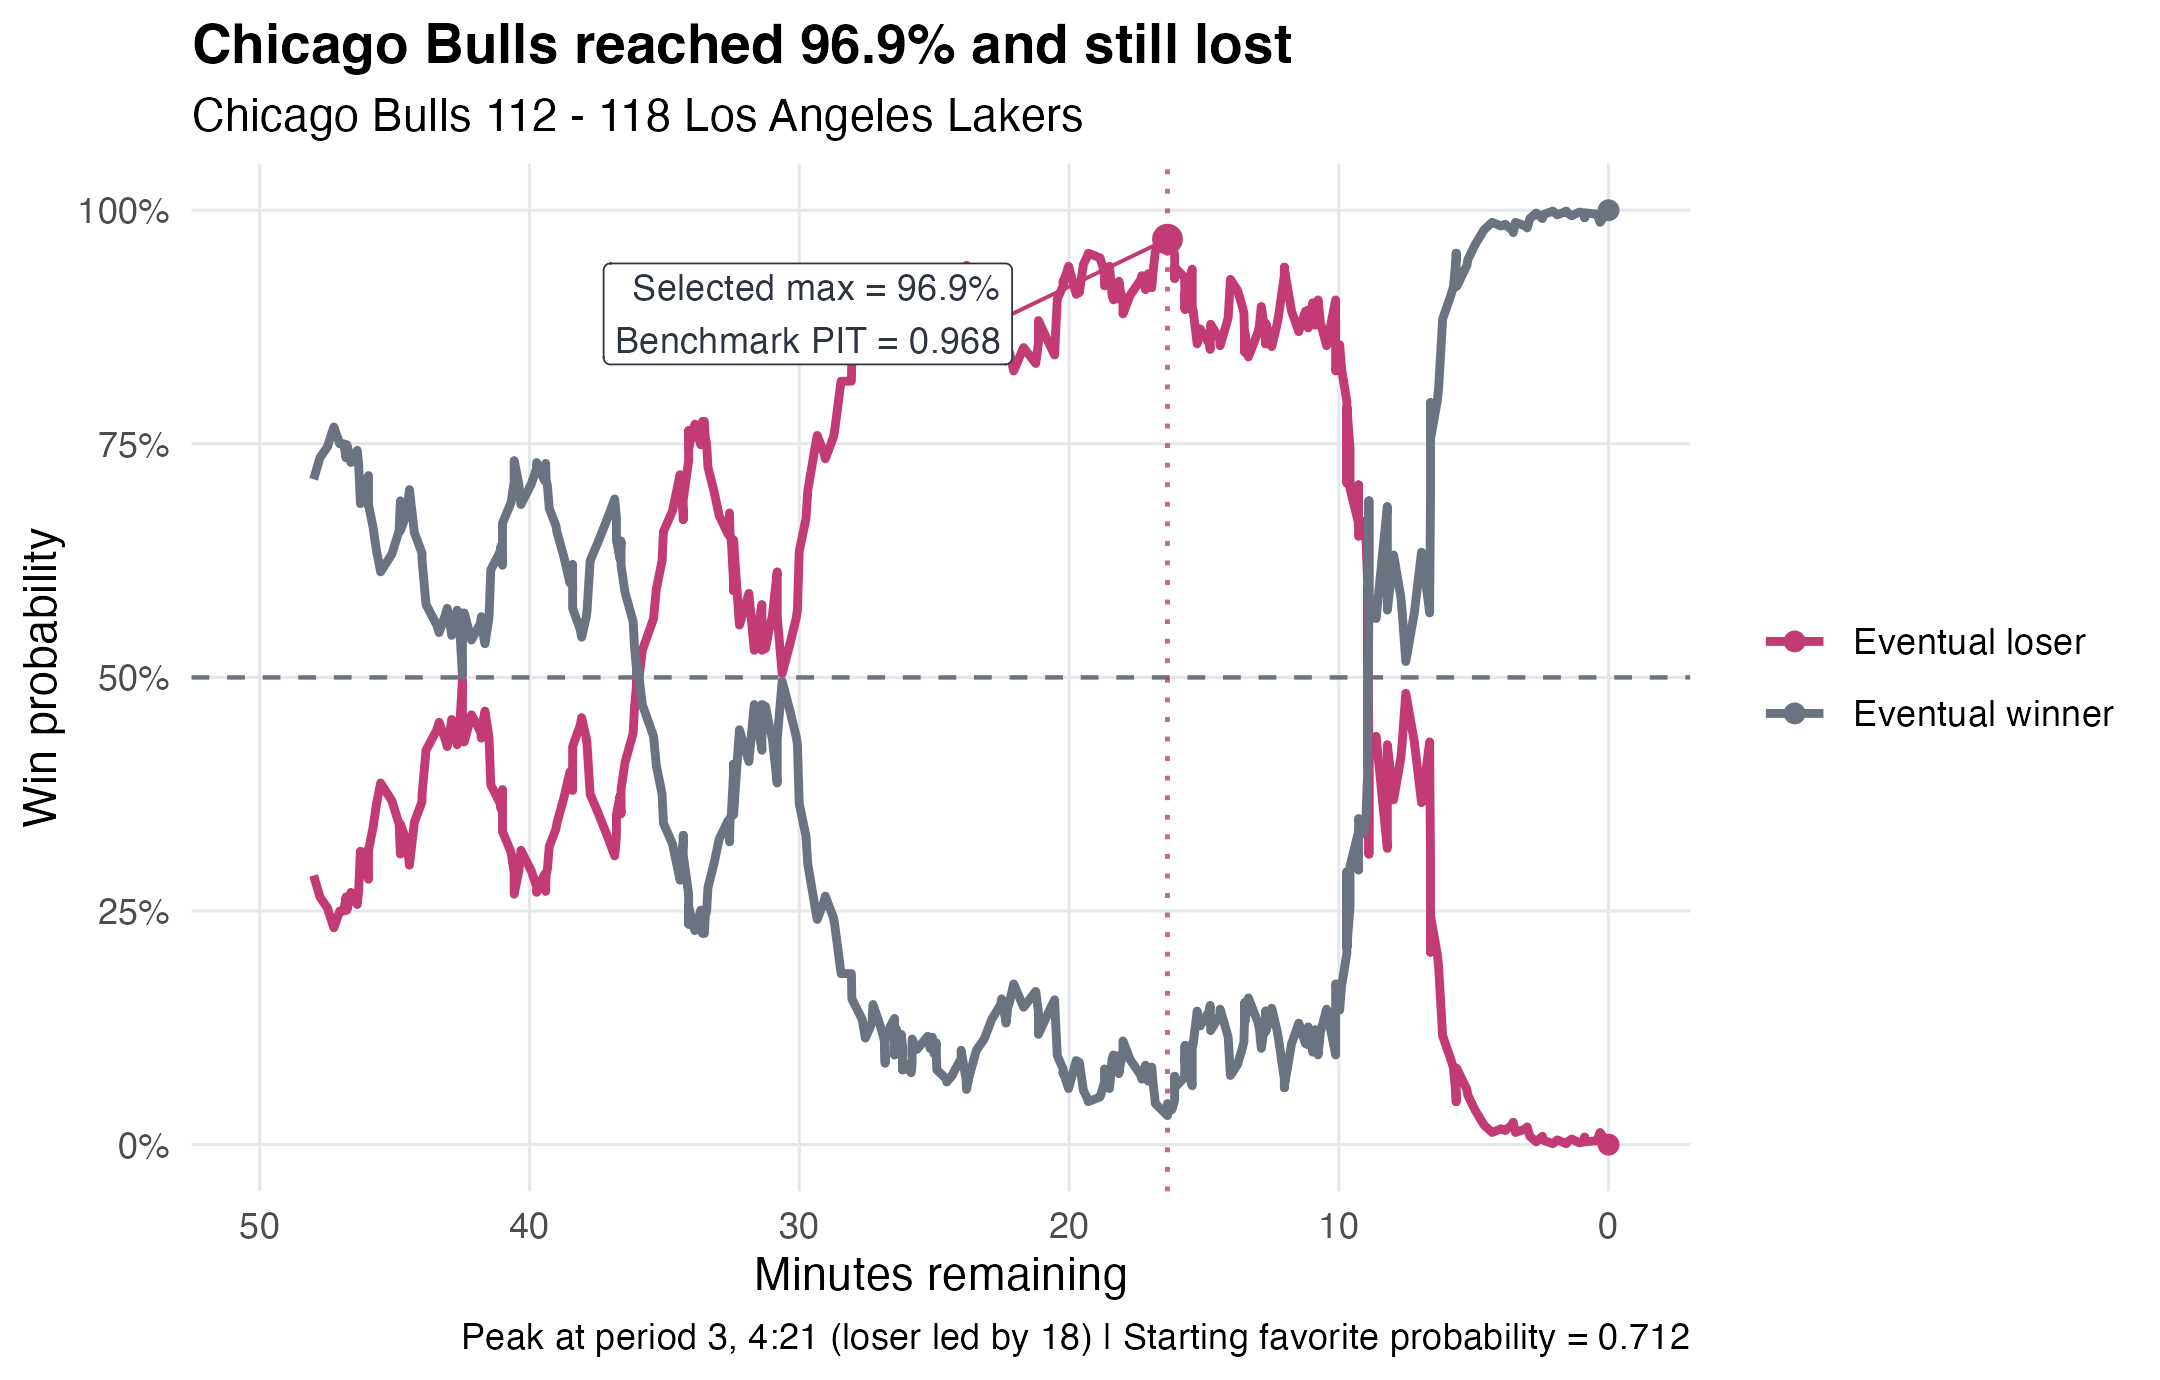
\includegraphics[width=0.92\textwidth]{figures/case_studies/nba_extreme_case_study.png}
\caption{Chicago's published win probability paths. The eventual loser's observed peak is \ChicagoMaxWP{} with \ChicagoMinutesRemaining{} minutes remaining; the game-specific benchmark maps that peak and $p_0=\ChicagoStartingWP$ to $U=\ChicagoPIT$.}
\label{fig:nba-extreme-case}
\end{figure}

Chicago is unusual even on this scale, but one game cannot diagnose a feed.
The league-level question is whether games at least this unusual recur at the rate the benchmark allows.
Supplementary Section~S4 gives benchmark values for other common thresholds.

\section{A league-level diagnostic} \label{sec:diagnostics}

Once a single game can be scored, the next question is how to compare many such games drawn from different starting conditions.
The benchmark CDF puts their losing-team peaks on a common scale; the distribution of those scores then reveals whether a feed produces too many severe collapses.

\subsection{Game-level PIT scores}

For game $i$, let $p_{0,i}$ be the first reported favorite probability and let $m_i$ be the observed maximum win probability assigned to the team that eventually lost.
The game-specific benchmark score is
\[
U_i := F_{M_\lambda}(m_i; p_{0,i}).
\]
We call $U_i$ the probability-integral-transform (PIT) score associated with the game-specific benchmark.
Thus $M_\lambda$ is the ideal continuous losing-team peak, $m_i$ is the observed published-path peak, $U_i$ scores one game, and $D_n^{\mathrm{upper}}$ below aggregates those scores across a league.
Large values of $U_i$ correspond to unusually severe collapses under the benchmark.
For example, $U_i=0.97$ means that the losing-team peak exceeds 97\% of benchmark realizations with the same starting favorite probability.

Under the continuous-path law, $U_i$ is $\mathrm{Unif}(0,1)$.
For a discretely reported feed, missed peaks move scores away from the upper tail, so an excess of large $U_i$ remains the direction of interest.

\subsection{Dependence-robust league inference}

At the league level, the question is whether the empirical distribution of the $U_i$ places too much mass near one.
Under the continuous-path benchmark, the scores are uniform even when starting probabilities vary from game to game.
Discrete reporting moves scores downward, so for $\alpha\in(0,1)$ the operative null is
\[
\P(U_i\ge 1-\alpha)\le \alpha.
\]
The global statistic follows that direction:
\[
D_n^{\mathrm{upper}}
  :=\sup_{0\le t\le1}\{t-\hat F_U(t-)\}.
\]
We call the curve $t-\hat F_U(t-)$ the centered PIT signature; $D_n^{\mathrm{upper}}$ is its maximum.
The left limit preserves the weak upper-tail convention when published probabilities create ties; computationally, we maximize $u-\hat F_U(u-)$ over the distinct observed scores.
A large value means that the empirical CDF accumulates too slowly because too much mass lies near one.

Recurring teams and repeat matchups create shared-team dependence within seasons.
We account for this shared-team dependence with a season-stratified version of the pigeonhole bootstrap \citep{Owen2007,DaveziesDHAultfoeuilleGuyonvarch2021}.
Within season $s$, let $W_{sa}$ be the multiplicity obtained by sampling that season's teams multinomially with replacement.
A game between teams $a$ and $b$ receives weight $W_{sa}W_{sb}$.
Thus repeat meetings share an endpoint weight, while normalization makes the total weight in each season equal its observed number of games.
The corresponding asymptotic argument assumes that each season is a jointly exchangeable, dissociated dyadic array: games may depend when they share a team but are independent when their endpoint sets are disjoint.
The multiple-observation extension of \citet{DaveziesDHAultfoeuilleGuyonvarch2021} allows both zero games and repeated games in a matchup cell.

For each of $B=\DyadicBootstrapReplicates$ draws, we recompute the weighted empirical CDF and form the centered statistic
\[
D_n^*=\sup_t\{\hat F_U(t)-\hat F_U^*(t)\}.
\]
The reported global $p$-value is
\[
\frac{1+\sum_{b=1}^B \mathbf 1\{D_{n,b}^*\ge D_n^{\mathrm{upper}}\}}{B+1}.
\]
Recentering measures how far a resampled CDF can fall below the observed CDF without carrying the observed departure into every replicate.
We pair this global test with an interpretable effect size,
\[
\Delta_{.95}:=\widehat{\P}_n(U\ge0.95)-0.05.
\]
Its uncertainty is summarized by a two-sided percentile interval from the same dyadic draws.
Under these conditions, the recentered pigeonhole bootstrap consistently estimates the CDF empirical process.
Together with $F_U(t-)\ge t$, this yields an asymptotically conservative upper-tail test.
Because this result is asymptotic, we assess finite-schedule behavior using simulations on the observed schedules.
Supplementary Section~S5 specializes the exchangeable-array bootstrap result to the normalized game-level CDF; Sections~S7--S8 report the dependence sensitivities and finite-schedule null simulation.

\section{Application to NFL and NBA win probability feeds} \label{sec:empirical}

We apply the game-level score separately to ESPN's public NFL and NBA win probability paths \citep{ESPN2025}.
The NFL data were assembled with \texttt{espnscrapeR} \citep{espnscrapeR2025}; the NBA data were assembled with \texttt{hoopR} \citep{hoopR2023}.
Both samples contain regular-season franchise games only, although the season labels follow league convention.
An NFL season is labeled by the year in which it begins, so games played the following January retain the preceding year's label; an NBA season is labeled by the year in which it ends.
Because ESPN's NBA season-type field also includes All-Star exhibitions, we additionally require both participants to be NBA franchises.
That filter removes \NBAExcludedExhibitionEvents{} All-Star or Rising Stars events, \NBAExcludedExhibitionFeeds{} of which had usable probability paths.
From the 2018--2024 season inventories, we retain completed games, exclude NFL ties, and require a usable published probability path.
Table~\ref{tab:data-coverage} shows the resulting coverage.

\begin{table}[!htbp]
\centering
\small
\caption{Regular-season feed construction. Eligible games are completed, non-tied games; analyzed games also have a usable public win probability path.}
\label{tab:data-coverage}
\begin{tabular}{lrrrrr}
\hline
League & Scheduled & Completed & Eligible & Analyzed & Missing feed \\
\hline
NFL & \NFLScheduledGames & \NFLCompletedGames & \NFLEligibleGames & \NFLGames & \NFLMissingFeedGames \\
NBA & \NBAScheduledGames & \NBACompletedGames & \NBAEligibleGames & \NBAGames & \NBAMissingFeedGames \\
\hline
\end{tabular}
\end{table}

Our estimand is ESPN's published feed, encompassing both forecast generation and the conversion of internal output into displayed probabilities.
For each game we retain the first published probability, the complete sequence of published updates, the final outcome, and the first attainment of the eventual loser's peak.
Overtime updates remain part of the collapse statistic because a collapse can occur in overtime.

The feeds are published at different resolutions.
The NFL sample contains \NFLPublishedUpdates{} updates, with a median of \NFLMedianUpdatesPerGame{} per game (interquartile range \NFLUpdateQOne--\NFLUpdateQThree); the NBA sample contains \NBAPublishedUpdates{}, with a median of \NBAMedianUpdatesPerGame{} (interquartile range \NBAUpdateQOne--\NBAUpdateQThree).
We preserve those resolutions because thinning a path can hide its maximum and change the estimand.
The leagues serve as parallel applications of the same benchmark, with each interpreted in the context of its own schedule, game dynamics, and publication resolution.

\subsection{Fixed-clock calibration}

Before asking how high the losing path ever rose, consider the more familiar question studied by \citet{YehRiceDubin2022}: at comparable points in a game, do published probabilities agree with observed win rates?
We adapt their calibration-surface idea to a common regulation clock.
Each game's home-team forecast is evaluated at $t=0,.05,\ldots,.95$ of regulation, using linear interpolation between published updates, with piecewise-constant interpolation as a sensitivity analysis.
At each time, ten adaptive probability bins are formed from empirical quantiles without splitting tied forecasts.
Every retained game therefore contributes once at each time rather than in proportion to its number of published updates.
Overtime is excluded from this common-clock display.
The complete fixed-clock samples contain \NFLFixedClockGames{} NFL games and \NBAFixedClockGames{} NBA games; \NBAFixedClockExcluded{} NBA paths end before the full grid and are excluded from this comparison only.

Figure~\ref{fig:fixed-clock-envelope} compresses the resulting calibration surfaces.
At each time, the dark region spans the observed-minus-forecast gaps across bins, and the lighter region spans their simultaneous dyadic-bootstrap limits.
In the full time--probability surfaces, the cells whose simultaneous intervals exclude zero are concentrated late in regulation and near published probabilities of zero or one in both applications (Supplementary Figure~S6.1).
The two diagnostics answer different questions: fixed-clock calibration evaluates forecasts at prespecified times, whereas the losing-path diagnostic selects a maximum after the loser is known.

\begin{figure}[!htbp]
\centering
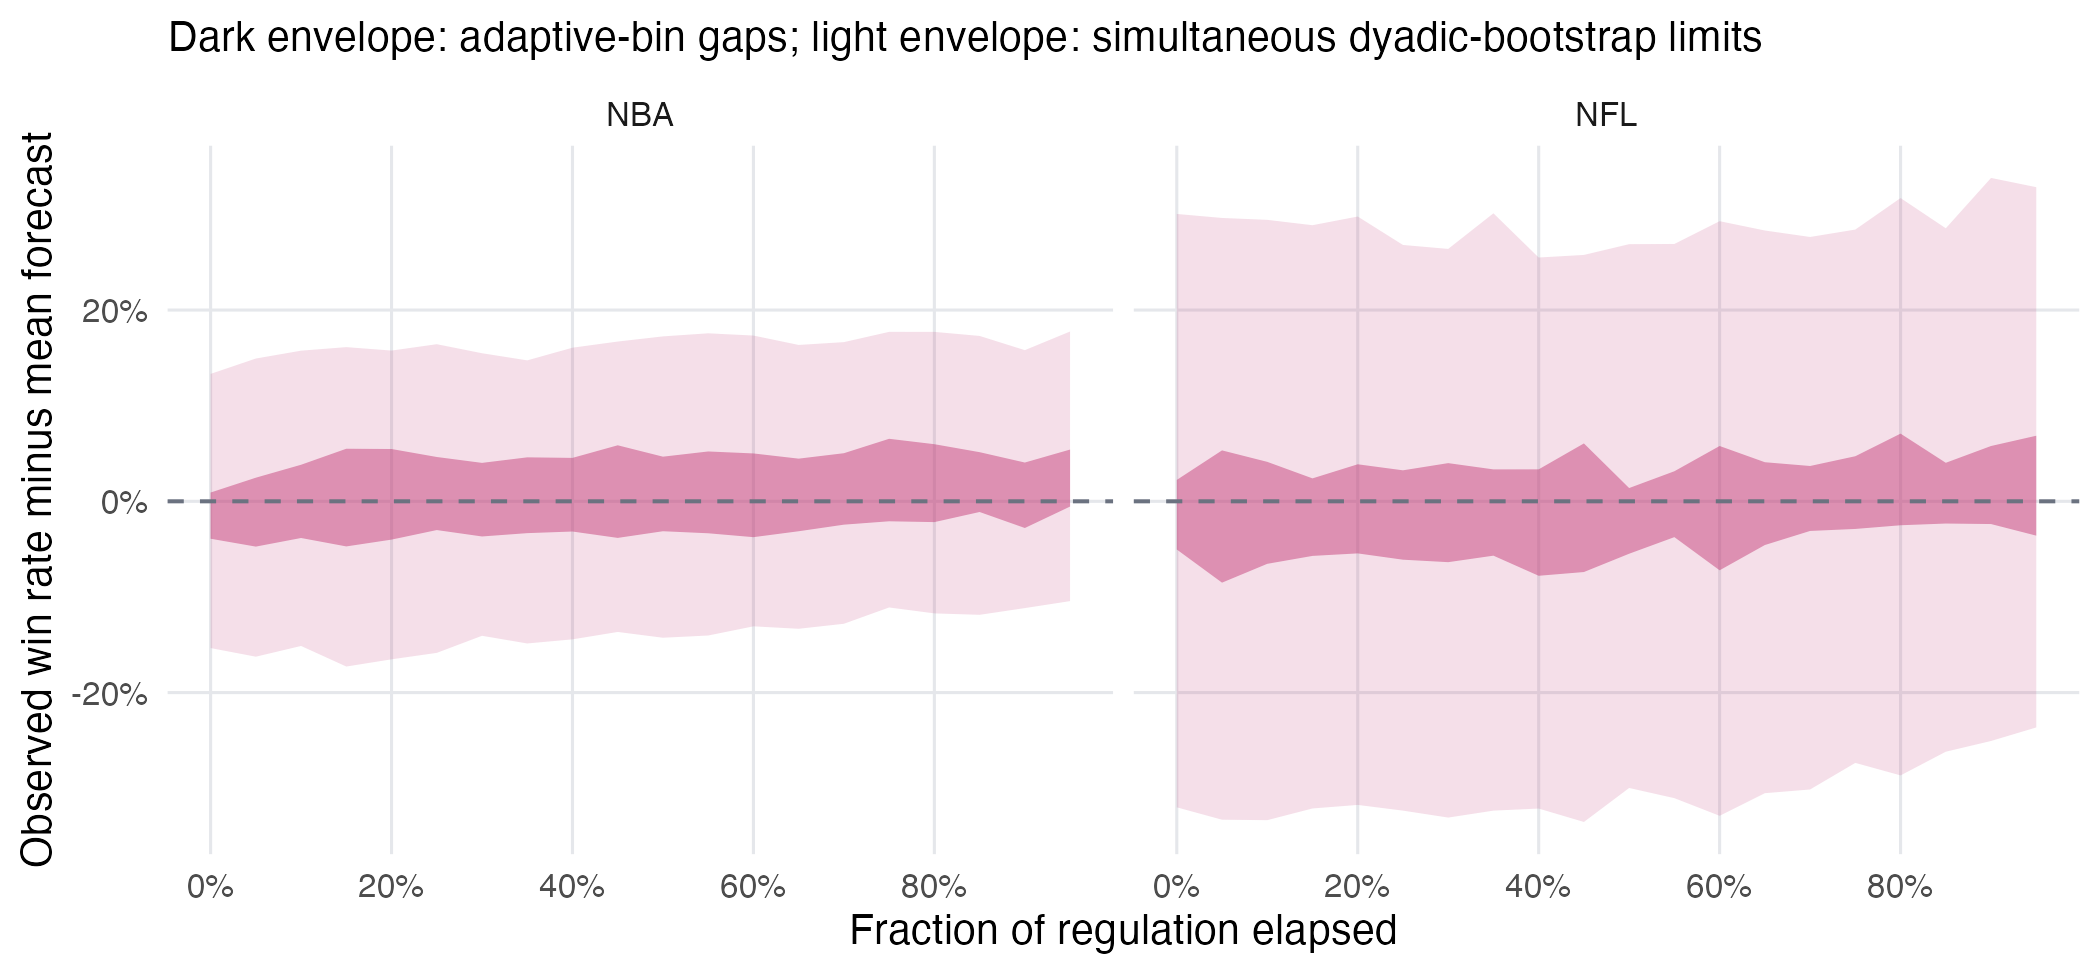
\includegraphics[width=0.95\textwidth]{figures/fixed_clock_calibration_envelope.png}
\caption{Fixed-clock calibration envelopes using linear interpolation. Each game contributes once at each fraction of regulation. Dark regions span the ten tie-preserving adaptive-bin gaps; light regions include the simultaneous season-stratified dyadic-bootstrap limits. Full time--probability surfaces and the LOCF sensitivity appear in the supplement.}
\label{fig:fixed-clock-envelope}
\end{figure}

\subsection{The losing-path diagnostic}

For each game, the losing-path diagnostic maps the eventual loser's peak $m_i$ through the game-specific benchmark CDF before aggregation.
Figure~\ref{fig:pit-combined} shows the resulting curves $t-\hat F_U(t-)$.
The dot-dash line in each panel marks the 95th percentile of the centered dyadic-bootstrap statistic used for formal inference.

\begin{figure}[!htbp]
\centering
\begin{minipage}[t]{0.8\textwidth}
  \centering
  
\includegraphics[width=\textwidth]{figures/nfl/pit.png}
  \smallskip\par\small (a) NFL
\end{minipage}\\[0.5em]
\begin{minipage}[t]{0.8\textwidth}
  \centering
  
\includegraphics[width=\textwidth]{figures/nba/pit.png}
  \smallskip\par\small (b) NBA
\end{minipage}
\caption{Centered PIT signatures $t-\hat F_U(t-)$ and the 95\% season-stratified dyadic-bootstrap critical value (dot-dash). The NFL application has no detected global departure; the NBA application exceeds its reference.}
\label{fig:pit-combined}
\end{figure}

\begin{table}[!htbp]
\centering
\small
\caption{Primary inference for each application. The interval is a two-sided percentile interval from the same season-stratified dyadic draws used for the global test.}
\label{tab:primary-inference}
\begin{tabular}{lccccc}
\hline
League & Games & $D_n^{\mathrm{upper}}$ & Dyadic $p$ & $\widehat{\P}(U\ge0.95)$ & $\Delta_{.95}$ (95\% CI) \\
\hline
NFL & \NFLGames & \NFLGlobalD & \NFLGlobalDyadicP & \NFLTailNinetyFiveRate & \NFLTailNinetyFiveExcess{} [\NFLTailNinetyFiveCILower, \NFLTailNinetyFiveCIUpper] \\
NBA & \NBAGames & \NBAGlobalD & \NBAGlobalDyadicP & \NBATailNinetyFiveRate & \NBATailNinetyFiveExcess{} [\NBATailNinetyFiveCILower, \NBATailNinetyFiveCIUpper] \\
\hline
\end{tabular}
\end{table}

The two applications diverge.
For the NFL, $D_n^{\mathrm{upper}}=\NFLGlobalD$ and the dyadic test gives $p=\NFLGlobalDyadicP$.
This conservative test yields no detected departure, leaving exact calibration unresolved.
For the NBA, $D_n^{\mathrm{upper}}=\NBAGlobalD$ and the upper-tail null is rejected ($p\NBAGlobalDyadicP$).
We use the global test to detect departure over the full score distribution and the $0.95$ tail to express its magnitude on a familiar scale.
In the NBA, \NBATailNinetyFiveRate{} of games occupy a benchmark tail of size $5\%$, an excess of \NBATailNinetyFiveExcess{} (95\% interval \NBATailNinetyFiveCILower{} to \NBATailNinetyFiveCIUpper{}).

\FloatBarrier
\subsection{First crossings of 0.95}

The event $U\ge0.95$ refers to the upper 5\% of the \emph{game-level collapse benchmark}; it is not the event that a published win probability crosses $0.95$.
The latter offers a more immediate view of where the discrepancy enters.
For a team-side path, define
\[
\tau_{.95}:=\inf\{k:p_k\ge0.95,\ \text{game time remaining}>0\}.
\]
If no preterminal crossing occurs, set $\tau_{.95}=N$.
Then $\tau_{.95}$ is a bounded stopping time and the crossing event $\{\tau_{.95}<N\}$ is known at that time.
Sequential calibration gives
\[
\E\!\left[(p_{\tau_{.95}}-Y)
  \mathbf 1\{\tau_{.95}<N\}\right]=0.
\]
Optional stopping therefore centers the selected preterminal first-crossing residual at zero under sequential calibration.
At a crossing, $1-p_{\tau_{.95}}$ is the implied loss probability and $1-Y$ is the loss indicator, so observed minus implied loss is
\[
R=(1-Y)-(1-p_{\tau_{.95}})=p_{\tau_{.95}}-Y.
\]

The NBA contributes \NBACrossingNinetyFiveEpisodes{} team-side episodes from \NBACrossingNinetyFiveGames{} games.
The observed loss rate is \NBACrossingNinetyFiveLoss{}, compared with a mean implied loss of \NBACrossingNinetyFiveImplied{}, leaving $\bar R=\NBACrossingNinetyFiveResidual$ (95\% interval \NBACrossingNinetyFiveCILower{} to \NBACrossingNinetyFiveCIUpper{}).
For the NFL, $\bar R=\NFLCrossingNinetyFiveResidual$ (\NFLCrossingNinetyFiveCILower{} to \NFLCrossingNinetyFiveCIUpper{}).
Every episode from the same game receives the same game weight, including the uncommon case in which both teams cross.
The crossing analysis shows that the NBA gap is already visible at the first entrance into a high-probability state.

\subsection{Sensitivity to feed artifacts}

The principal artifact checks change one feature at a time while reusing the same bootstrap draws.
For the NBA, $D_n^{\mathrm{upper}}$ is \NBAGlobalD{} on corrected paths, \NBARawGlobalD{} on raw paths, and \NBAExcludePatchedGlobalD{} after removing all \NBAPatchedGames{} games in which the feed incorrectly assigned probability one to the eventual loser.
Allowing each displayed probability to lie within $\pm0.0005$ bounds $D_n^{\mathrm{upper}}$ between \NBARoundingLowerGlobalD{} and \NBARoundingUpperGlobalD{}.
The dyad-plus-calendar sensitivity gives $p\NBADyadicCalendarGlobalP$, and the franchise-linked cross-season sensitivity gives $p\NBAFranchiseLinkedGlobalP$.
Leaving out one season at a time yields NBA statistics from \NBALOSODMin{} to \NBALOSODMax{}.
The NFL continues to show no detected departure under the corresponding corrections, rounding bounds, calendar blocks, franchise linkage, and season omissions.

Coverage is complete for the NFL and at least \NBAMinimumFeedCoverage{} in every NBA season.
Supplementary Section~S7 collects the full specification table, including boundary and terminal conventions, the $0.90$, $0.95$, and $0.99$ tail and crossing results, and leave-one-season-out analysis.
Section~S6 gives the full fixed-clock surfaces, LOCF sensitivity, and season-level feed inventories.

\section{Effect of discrete reporting} \label{sec:simulation}

The continuous benchmark is exact, but a public feed reveals only a finite set of points on the path.
Theorem~\ref{thm:discrete-conditional} says that discrete reporting can hide the true maximum and make the upper-tail diagnostic conservative.
The following simulation makes that direction visible.

For trajectory $i$, draw $p_{0,i}\sim\mathrm{Unif}(0.25,0.75)$ and $Y_i\sim\mathrm{Bernoulli}(p_{0,i})$.
With an independent standard Brownian bridge $B_i^0$, define
\[
X_i(t)=tY_i+\sigma B_i^0(t),\qquad \sigma=0.5,
\]
and, for $t<1$,
\[
p_i(t)=\operatorname{logit}^{-1}\!\left\{
\operatorname{logit}(p_{0,i})+
\frac{X_i(t)-t/2}{\sigma^2(1-t)}
\right\},
\qquad p_i(1)=Y_i.
\]
Here $p_i(t)$ is the posterior probability that the bridge ends at one given the signal observed through time $t$, so it satisfies the sequential-calibration ideal.
We simulate the process on a grid with $K_{\mathrm{base}}=\SimulationBaseGrid$ points, then retain every $m$th report before computing the eventual loser's maximum and benchmark score.

Figure~\ref{fig:sim-null-gap} shows the consequence.
As reports become less frequent, $t-\hat F_U(t-)$ moves downward.
Coarsening removes opportunities to observe a high losing-team peak and therefore works against upper-tail rejection.

\begin{figure}[!htbp]
\centering

\includegraphics[width=0.9\textwidth]{figures/simulation/null_conservatism.png}
\caption{Centered PIT signatures after observing a common calibrated process at progressively coarser resolutions ($K_{\mathrm{base}}=\SimulationBaseGrid$). Coarsening makes the upper-tail benchmark conservative.}
\label{fig:sim-null-gap}
\end{figure}

\FloatBarrier
\section{Discussion} \label{sec:discussion}

A blown lead poses two questions: at $90\%$, calibration compares outcomes across similar forecasts; after the game, the selected loser's maximum is judged against the law of losing-team maxima.
That second benchmark turns a familiar sports claim into a testable statement about a published forecast sequence.
In our applications, the NFL feed shows no detected global departure, while the NBA feed contains too many extreme losing-team peaks.
The NBA departure characterizes the published feed; model specification, the effective information set, league dynamics, and the publication process can all contribute.

\subsection{Limitations and assumptions}

Our theoretical benchmark concerns the ideal process $p_k=\E[Y\mid\mathcal F_k]$.
Published win probabilities approximate this conditional expectation using an effective information set that may differ from the outcome-relevant filtration.

The exact identities additionally require continuous sample paths, which preclude first-passage overshoots and, below one, terminal-time first attainment.
For discretely reported feeds, the bounds remain valid; the explicit correction terms measure the effects of overshoots and terminal attainment.
Finally, we treat binary terminal outcomes $p_N\in\{0,1\}$; extensions to ties or other non-binary terminal structures require different arguments.

The empirical intervals describe games and matchups in the observed 2018--2024 regular seasons.
With seven season labels, season-to-season persistence is summarized descriptively.
Weak or degenerate shared-team dependence can make the pigeonhole bootstrap conservative \citep{Menzel2021}.
The finite-schedule null simulation evaluates Type I error under shared-team dependence, while franchise-linked and calendar-block sensitivities probe dependence beyond the primary dyadic model.

The Chicago game contributes one severe score, $U=\ChicagoPIT$; the recurrence of similarly extreme losing paths across \NBAGames{} NBA games is what turns a memorable collapse into evidence about a published forecasting system.


\begin{acks}[Acknowledgments]

We thank Jiaoyang Huang, Ryan Brill, and Paul Sabin for helpful discussions and feedback.

\end{acks}

\begin{supplement}
\stitle{Supplementary Material for The Blown Lead Paradox}
\sdescription{Proofs, dependence and bootstrap justification, full data and calibration documentation, robustness analyses, and finite-schedule validation.}
\end{supplement}

\bibliographystyle{imsart-nameyear}
\bibliography{references}
\end{document}
